\documentclass{article}

\usepackage{hyperref}
\usepackage{pdfpages}

\title{Ring VRFs from zk continuations: \\ Ethical identity and anonymous rationing}
\author{Jeffrey Burdges \and Handan Kilinc-Alper \and Alistair Stewart \and Sergey Vasilyev}
\date{}

\begin{document}

\maketitle


\paragraph{Abstract:} \quad 

A {\it ring verifiable random function} (ring VRF) is a ring signature
that proves correct evaluation of some pseudo-random function (PRF)
determined by the actual key pair used in signing, but while hiding
the actual signer's identity within some set of possible signers,
known as the ring.

\smallskip

We show ring VRFs that amortize their ring membership proof across many
ring VRF signatures.
%
For this, we devised a {\em zero-knowledge continuation} technique that
reuses a previously proven Groth16 SNARK without reproving.
We wire this Groth16 SNARKs inputs into another signature, or another SNARK, 
but avoid linking the multiple reuses by adjusting the Groth16 trusted setup
to reblind the public inputs when rerandomizing the Groth16.
%
Incredibly, our ring VRF needs only eight $\mathcal{G}_1$ and two
$\mathcal{G}_2$ scalar multiplications, irregardless of the ring size!

\smallskip

Ring VRFs provide a flexible  but straightforward framework to address
diverse deployment and privacy problems, so they could truly bring
anonymous credentials into the main stream.

Ring VRFs produce a unique identity for any give context but remain
unlinkable between different contexts.  These unlinkable but unique
pseudonyms provide a far better balance between user privacy and service
provider or social interests than attribute based credentials like IRMA.

Ring VRFs support anonymously rationing or rate limiting resource
consumption that winds up vastly more efficient than purchases via
money-like protocols.  Importantly ``rings'' are far cleaner to audit
than certificates, in principle reducing fraud and improving trust.

We discuss anonymous credentials face malicious verifier problems,
but how ring VRF inputs could include their root of trust, which
avoids third party CAs and complexities like certificate transparency.


\paragraph{Proposal:} \quad

Jeffrey Burdges would love to present our zero-knowledge continuation
technique, how it enables extremely efficient ring verifiable
random functions (ring VRFs).

In this, Jeff would focus primarily upon how ring VRFs yield one of the
safest identity schemes, as well as their applications to rate limiting,
including the idea of anonymous ration cards.

\smallskip

At \quad \url{https://www.youtube.com/watch?v=0i_5RW3tkVM} \quad you'll
find Jeff's 20 minute talk on this material at the
ZK Summit in Berlin.

\smallskip

For RWC, Jeff envisions doing a more polished talk, which better clarifies
the problem space, and focuses more on ring VRF input structure,
specifically:
\begin{itemize}
\item The abuse risks of attribute based credentials like
 IRMA (``I Reveal My Attributes'') credentials.
 And why ring VRFs yield a safer identity scheme.
\item How verifier abuse demands verifier certification, which IRMA does
 not address, but ring VRFs do.  In particular, a root key in the VRF input
 permits certifying verifiers without adding CA complexities.
\item We'll better describe how a ``ring'' based credential improves
 the audit trail, and hence user trust, over anonymized certificate schemes
 like IRMA.  We think this becomes extremely important if used for rationing,
 as anonymous credentials won't admit analogs of certificate transparency.
\end{itemize}

\noindent Additional refinements include:
\begin{itemize}
\item An RWC audience likely wants clearer, but not deeper, comments
 on the trusted setup than required for ZK Summit.
\item We regret abandoning its jokes, but we shall omit our secret single
 leader election (SSLEs) application Sassafras, as it takes us too far
 away from the privacy story, and RWC's audience feels less interested in
 consensus protocols.  We'll see if cards against humanity still fits.
\item We repeatedly cautioned the blockchain heavy ZK Summit audience
 that zero-knowledge continuations cannot amortize crypto-currency
 UTXOs, but this feels unnecessary for a RWC audience.
\end{itemize}


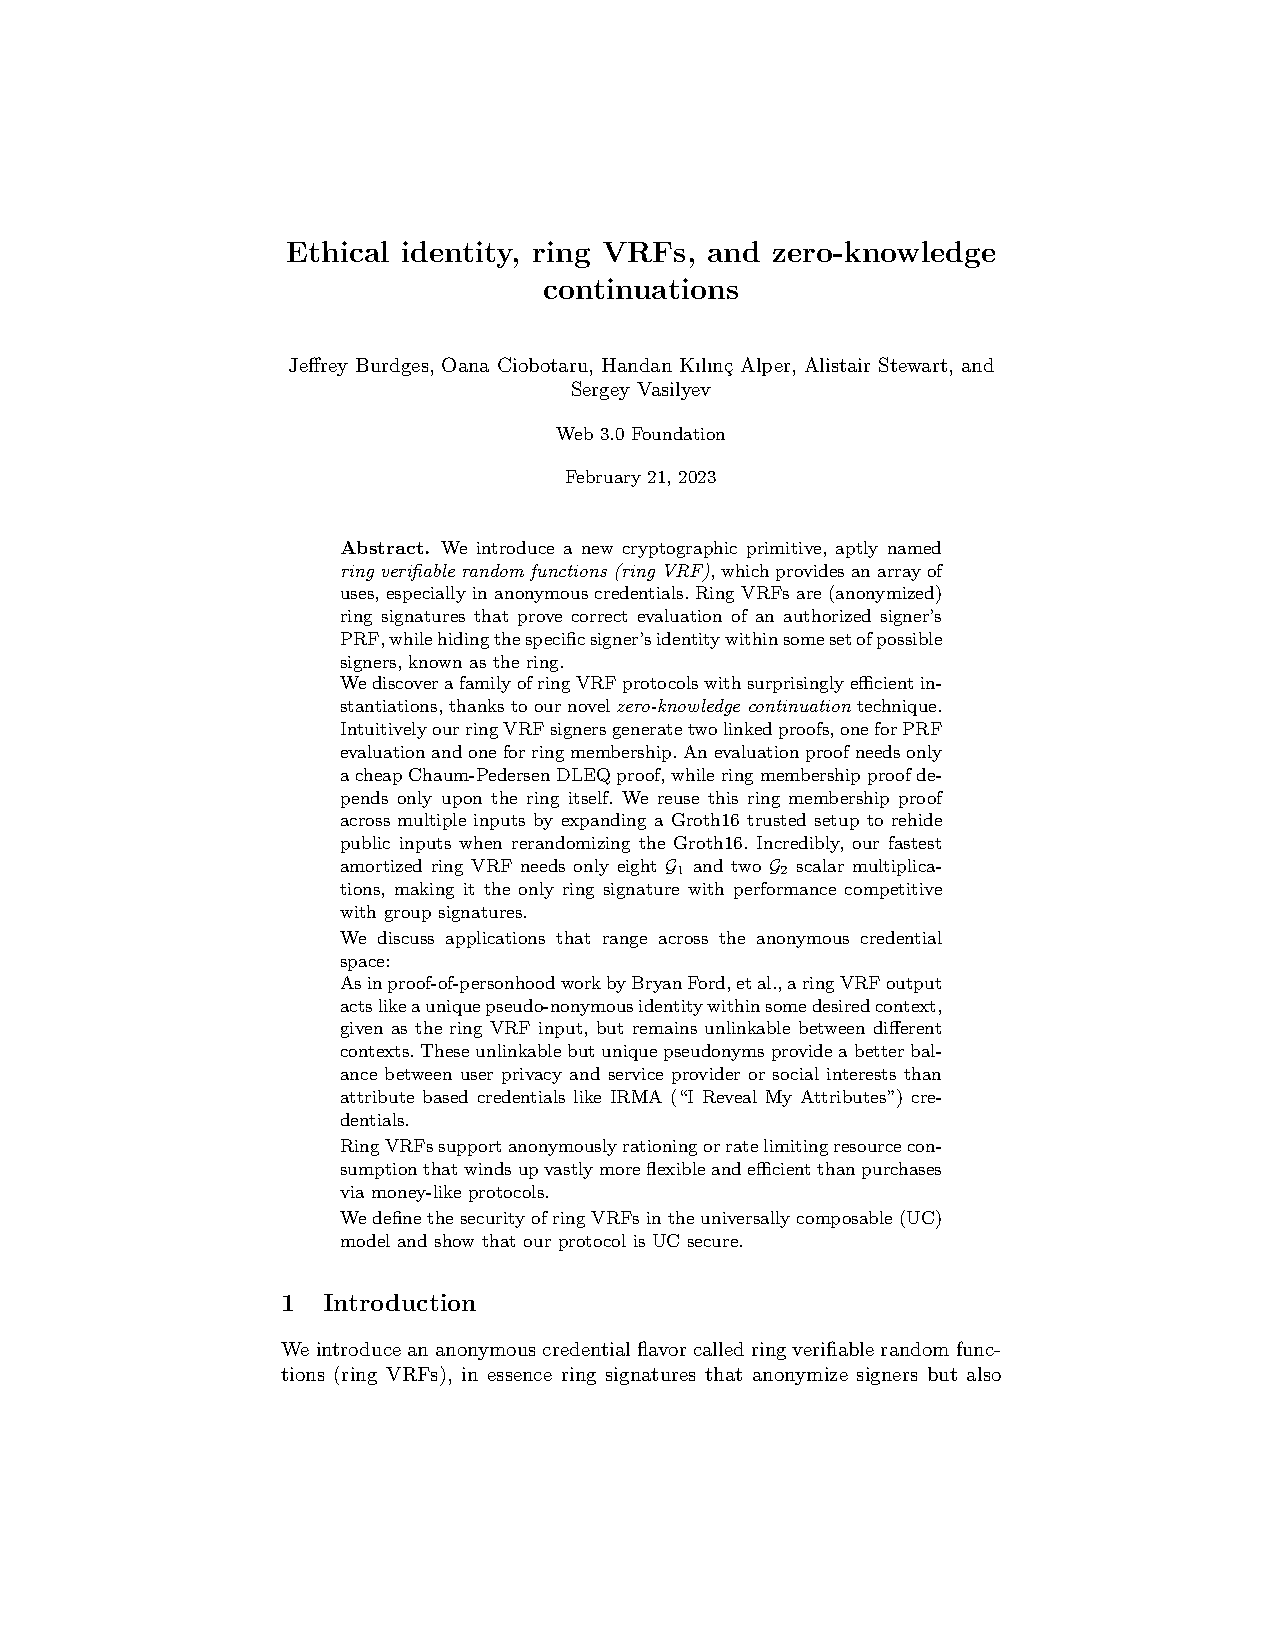
\includepdf[pages=-]{ring_vrf.pdf}


\end{document}


\endinput



\smallskip

Our zero-knowledge continuation reuses a previously proven Groth16 SNARK
without reproving.  We wire this SNARKs inputs into another signature,
or another SNARK, without linking the multiple reuses.

\smallskip

Almost all prover time could therefore by amortized away by the application,
dramatically improving performance.  In particular, our ring VRF has a marginal
prover CPU cost of roughly 12 scalar multiplications!

